\chapter{Background: Browser Fingerprinting}

Browser fingerprinting is a method of identifying users by gathering information about their browser.
When a user visits a website which employs browser fingerprinting strategies, the website will both passively and actively collect information about the user's browser.
When the user returns to the site, the browser characteristics can be checked and compared with previous users' fingerprints \citep{fingerprinting}.
This way, a match can be found and the user can be uniquely identified.

Some of the information is gained `passively' as it is sent in the HTTP request.
The other information is `actively' gathered through client-side JavaScript, Flash and Java execution.

\subsection{Passively Gained Information}

HTTP requests sent to websites offer much information about the user.
The browser exposes this data by setting the values of certain request headers.
The first relevant header is User Agent.
This is a string which normally details what browser, platform and layout engine are being used, along with the versions of each (see Figure~\ref{fig:useragent-example} for an example).
This is done so that websites can identify interoperability problems more easily \citep{useragent}.
The user agent carries approximately 10.5 bits of identifying information on average, exposing a substantial amount of information to visited websites \citep{useragententropy}.

\begin{figure}[h]

\includegraphics[scale=0.8]{useragent-example}
\centering
\caption{Example of a user agent}
\label{fig:useragent-example}
\end{figure}

The next relevant headers are the HTTP\_\_ACCEPT headers.
These describe what MIMETYPE the browser is looking for, what compression formats it will accept and what languages are desired.

\begin{figure}[h]

\includegraphics[scale=0.8]{http-accept-example}
\centering
\caption{Example of HTTP\_\_ACCEPT headers}
\end{figure}

As well as the previous headers, the browser will also send the date of the machine, including the timezone.
This exposes both the timezone that the user is located in, and the time difference between the client machine and the server.
There is one last header that is commonly used in fingerprinting, the DNT or `Do Not Track' header.
This header is a binary value which indicates to a website if the user explicitly does not want to be tracked.

All of this information is sent by default, exposing a huge amount of data about the user's browser already.
Furthermore, much of this data is important for user experience on a lot of websites, such as websites with downloads for different operating systems checking the User Agent string to show a different download for different operating systems.
This means that spoofing the data to protect the user's privacy comes with a common tradeoff, user experience vs.\ privacy.

\subsection{Actively Gained Information}

As well as the information that's sent to websites by the browser by default, there's also a huge amount of information that can be gleamed through client-side execution of JavaScript, Flash and Java.
One of the most reliable methods of mitigating fingerprinting is simply disabling all three of these, however most popular websites use JavaScript in some capacity and will either break the website entirely or result in a poor user experience \citep{disable-js}.

\subsubsection{Information Gained Using JavaScript}

JavaScript exposes a huge amount of information to fingerprinters.
A lot of the information is stored in the \texttt{window.navigator} JavaScript object which is available to any website that a user visits with JavaScript enabled.
This information is explained in Table~\ref{tab:navigator-props}.

\begin{table}[h]
\centering
\begin{tabular}{| l | r |}
    \hline
    \textbf{Navigator Property} & \textbf{Description} \\ \hline
    \texttt{appVersion} & {Returns the version of the browser} \\ \hline
    \texttt{cookieEnabled} & {Returns whether or not cookies are enabled} \\ \hline
    \texttt{javaEnabled()} & {Returns whether or not Java is enabled} \\ \hline
    \texttt{language} & {Returns the language of the browser} \\ \hline
    \texttt{platform} & {Returns the browser platform / operating system} \\ \hline
    \texttt{plugins} & {Returns the list of plugins installed in the browser} \\ \hline
    \texttt{product} & {Returns the product name of the browser engine} \\ \hline
    \texttt{userAgent} & {Returns the User Agent of the browser} \\
    \hline
\end{tabular}
\caption{Relevant \texttt{window.navigator} Properties}
\label{tab:navigator-props}
\end{table}

The most significant of these properties in terms of bits of entropy exposed is the \texttt{plugins} property, since it varies quite significantly from browser to browser.
It returns the list of plugins installed, usually paired with the version.
However, this list is not fully enumerable, it can not be read as one would expect.
To check if a user has a plugin installed, the fingerprinter must query the list with a specific plugin.
In addition to the characteristics available through the \texttt{window.navigator}, there are other objects with information available in them, such as the \texttt{screen} object which contains the height and width of the user's display.

Whereas these characteristics are convenient to access with JavaScript and readily supplied by the browser, there is also a huge amount of additional information which can be retrieved.
The first of which is detecting what fonts the user has installed.

Browsers and JavaScript do not supply any functions for retrieving the full list of fonts that the user has installed.
There is however a method that allows the visited website to detect what fonts are installed by querying a large number of fonts one-by-one.
The method works by creating a HTML \texttt{<span>} element and to set the font to a font that is known to be installed.
After this is done, JavaScript is used to change the CSS of the text so that the font family is different.
The size of the \texttt{<span>} element will be different before and after the change if the probed font is installed, illustrated in Figure~\ref{fig:font-change}.
A huge list of fonts can be tested for using this method, bypassing the inherent security feature of browsers not allowing full font enumeration.

\begin{figure}[h]
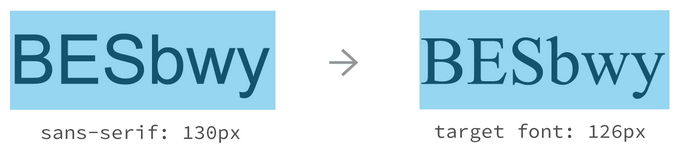
\includegraphics[scale=0.8]{font-change}
\centering
\caption{Difference in \texttt{<span>} width when the font is changed}
\label{fig:font-change}
\end{figure}

More information is exposed with some of the JavaScript \texttt{math} library functions.
A number of \texttt{math} library funcions will return different values depending on 32bit vs 64bit architectures, as well as what the operating system is.
For example, the output of \\
\texttt{Math.tan(-1e300)} is \texttt{-1.4214488238747245} on a 64bit Linux computer whereas it'll output \texttt{-4.987183803371025} on a Windows machine \citep{floating-point-bug}.
This basic test is one of the methods fingerprinters can use to check if a browser is spoofing its platform or User Agent.

There are two more important methods of gaining information about the browser through JavaScript, both similar in their approach.
The first is called `canvas fingerprinting'.
This works by using the \texttt{canvas} HTML element on a webpage.
A \texttt{canvas} element is a box on a webpage that text and graphics can be drawn to.
This rendered data can then be retrieved and sent back to the server.
Depending on a number of characteristics, such as the installed GPU and the graphics card drivers, this data will render slightly differently, exposing more information as a result \citep{canvas-fingerprint}.
This information is also orthogonal to other fingerprint information, consistent, high-entropy, is transparent to the user and is easily obtainable.

\begin{figure}[h]
\fbox{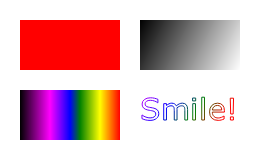
\includegraphics[scale=0.8]{canvas-example}}
\centering
\label{fig:canvas-example}
\caption{Example of a HTML5 \texttt{<canvas>} element}
\end{figure}

There's another similar method of fingerprinting called `audio fingerprinting'.
This uses the \texttt{AudioContext} browser API to generate and modify an audio signal.
This audio signal can be retrieved and measured, and once again differences between browsers are evident when comparing generated signals across different browsers.
It also reveals a number of other characteristics such as sample rate, max channel count and number of inputs and outputs \citep{audio-fingerprint}.

It's also possible to fingerprint the user by detecting the timing of keystrokes, since many users will have different typing patterns \citep{keystrokes}.

\subsubsection{Information Gained Using Flash}

The Flash plugin is a large source of browser information for fingerprinters.
Through Flash, the fingerprinter has access to the list of plugins the user has installed.
Unlike the \texttt{window.navigator} JavaScript object which also supplies the list of installed plugins, accessing the list through Flash fully enumerates the entire list and is fully readable, making it much easier to see the installed plugins.
As well as fully enumerating plugins, it also fully enumerates fonts.
Whereas in JavaScript, each font has to be queried individually, effectively limiting the number of fonts a fingerprinter can quickly check, Flash returns the full list of fonts that are installed on the system.
This makes it far easier to read the list of fonts and generally will give a much more in-depth list than probing for them using JavaScript.
This list of fonts can also be retrieved using a Java Applet.

Flash also exposes platform information, showing more information than the \texttt{window.navigator} JavaScript object as it shows the major and minor versions of the operating system instead of just the name and architecture.
In addition, Flash reveals the platform's language which isn't available through common browser APIs (Internet Explorer being the exception).

\subsection{Effectiveness of Browser Fingerprinting}

Given all of this information, one has to wonder just how useful it is in identifying browsers and consequently users.
According to a study done by the Electronic Frontier Foundation \citep{browser-uniqueness} using their Panopticlick fingerprinting tool, around 90\% of users who used the site to find their own fingerprint are unique.
This includes iPhone and Android browsers which are a lot more difficult to fingerprint due to the small amount of plugins and fonts that are commonly installed or available.
However, due to limited cookie options on these browsers they're often easier to track.
The most identifying characteristics were found to be plugins and fonts, followed by User Agent, HTTP Accept headers and screen resolution.
The 90\% figure may also be lower than the expected result for a more global sample because the type of user that would visit EFF's website are far more likely to already be privacy aware and use common browsers and plugins.

